% elementos pós-textuais 
\postextual

% apêndice 
\begin{apendicesenv}
\partapendices

% Apêndice A
\chapter{DEMONSTRAÇÕES} \label{apendice_a}

% lema 1
\begin{lemma}[condição de ausência de viés em $\mathbfit{\tilde{y}}$]
  \label{lema1}

  Se as previsões reconciliadas são não viesadas, então $\mathbfit{SGS=S}$, ou seja, $\mathbfit{G}$ é inversa generalizada de $\mathbfit{S}$.

\end{lemma}

\begin{proof}
  \begin{equation} \label{eq:ap1}
    \mathbfit{\tilde{y}}_{t+h|t} = \mathbfit{SG\hat{y}}_{t+h|t} 
  \end{equation}

  Se $\mathbfit{\hat{y}}_{t+h|t}$ é não viesado, então 

  \begin{equation} \label{eq:ap2}
      \mathbb{E}[\mathbfit{\hat{y}}_{t+h|t}] = \mathbb{E}[\mathbfit{y}_{t+h|t}] = \mathbfit{Sb}_t
  \end{equation}

  Da mesma forma, se espera-se que as previsões reconciliadas não sejam viesadas,
  \begin{equation} \label{eq:ap3}
      \mathbb{E}[\mathbfit{\tilde{y}}_{t+h|t}] = \mathbb{E}[\mathbfit{y}_{t+h|t}] = \mathbfit{Sb}_t
  \end{equation}

  Substituindo \eqref{eq:ap2} em \eqref{eq:ap1}, temos

  \begin{equation} \label{eq:ap4}
      \mathbfit{\tilde{y}}_{t+h|t} = \mathbfit{SGSb}_t 
  \end{equation}

  Logo, para manter a igualdade entre \eqref{eq:ap1} e \eqref{eq:ap4}, $\mathbfit{SGS=S}$

\end{proof}

% lema 2
\begin{lemma}
  \label{lema2}

  $\mathbfit{\tilde{e}}_t = \mathbfit{SG\hat{e}}_t$.

\end{lemma}

\begin{proof}
  \begin{equation} \label{eq:apa22}
    \mathbfit{\tilde{e}}_{t+h|t} = \mathbfit{y}_{t+h} - \mathbfit{\tilde{y}}_{t +h|t}
  \end{equation}

  Substituindo \eqref{eq:ap1} em \eqref{eq:apa22},

  \begin{align} \label{eq:apa23}
    \mathbfit{\tilde{e}}_{t+h|t} &= \mathbfit{y}_{t+h} - \mathbfit{SG\hat{y}}_{t+h|t}
  \end{align}

  Lembrando que, por definição, $\mathbfit{y}_{t+h} = \mathbfit{\hat{y}}_{t+h|t} + \mathbfit{\hat{e}}_{t+h|t}$, então

  \begin{align} \label{eq:apa24}
    \mathbfit{\tilde{e}}_{t+h|t} &= \mathbfit{\hat{y}}_{t+h|t} + \mathbfit{\hat {e}}_{t+h|t} - \mathbfit{SG\hat{y}}_{t+h|t} \\
    &= \mathbfit{\hat{e}}_{t+h|t} + \mathbfit{\hat{y}}_{t+h|t}(\mathbfit{I-SG)}
  \end{align}

  Usando a definição novamente, temos que

  \begin{align}
    \mathbfit{\tilde{e}}_{t+h|t} &= \mathbfit{\hat{e}}_{t+h|t} + (\mathbfit{y}_ {t+h} - \mathbfit{\hat{e}}_{t+h|t})(\mathbfit{I-SG)} \\
    &= \mathbfit{y}_{t+h} - \mathbfit{SGy}_{t+h|t} + \mathbfit{SG\hat{e}}_{t+h| t} \\
    &=  \mathbfit{y}_{t+h}(\mathbfit{I-SG}) + \mathbfit{SG\hat{e}}_{t+h|t}  \label{eq:apa25}
  \end{align}

  Substituindo \eqref{eq-vetor_b} em \eqref{eq:apa25}, temos

  \begin{align}
    \mathbfit{\tilde{e}}_{t+h|t} &=  \mathbfit{Sb}_{t+h}(\mathbfit{I-SG}) +  \mathbfit{SG\hat{e}}_{t+h|t} \\
    &=  \mathbfit{Sb}_{t+h} - \mathbfit{Sb}_{t+h}\mathbfit{SG} + \mathbfit {SG\hat{e}}_{t+h|t}  \\
    &=  \mathbfit{Sb}_{t+h} - \mathbfit{(G'S')(b'}_{t+h}\mathbfit{S')} +   \mathbfit{SG\hat{e}}_{t+h|t}  \\
    &=  \mathbfit{Sb}_{t+h} - \mathbfit{SG}\mathbfit{Sb}_{t+h} + \mathbfit {SG\hat{e}}_{t+h|t}
  \end{align}

  Finalmente, pela \nameref{lema1}, temos que

  \begin{align}
    \mathbfit{\tilde{e}}_{t+h|t} &=  \mathbfit{Sb}_{t+h} - \mathbfit{Sb}_{t+h}  + \mathbfit{SG\hat{e}}_{t+h|t}  \\
    &= \mathbfit{SG\hat{e}}_{t+h|t}
  \end{align}
\end{proof}

% teorema 1
\begin{theorem}
  \label{teorema1}

  $\text{Var}[\mathbfit{\tilde{e}}_t] = \mathbfit{SG\hat{W}G'S'}$.

\end{theorem}

\begin{proof}
  Por \ref{lema2}, temos que

  \begin{align}
    \text{Var}[\mathbfit{\tilde{e}}] &= \mathbb{E}[\mathbfit{(SG\hat{e})(SG\hat {e})'}] \\
    &= \mathbb{E}[\mathbfit{SG\hat{e}\hat{e}'G'S'}] \\
    &= \mathbfit{SG\hat{W}G'S'}
  \end{align}

  Em que $\mathbfit{\hat{W}}$ é a matriz de variância-covariância dos erros de  previsão base.
\end{proof}

\end{apendicesenv}

% anexos 
\begin{anexosenv}
\partanexos

\chapter{código para construção da base de dados} \label{anexo_a}

\begin{lstlisting}[frame=single]
  # pacotes
  library(magrittr, include.only = "%>%")
  
  # municípios x regiões imediatas
  municipios = basedosdados::read_sql("
  SELECT
    id_municipio
    , nome
    , nome_mesorregiao
    , nome_microrregiao
    , nome_regiao
    , nome_regiao_imediata
    , nome_regiao_intermediaria
  FROM `basedosdados.br_bd_diretorios_brasil.municipio`
  WHERE sigla_uf = 'ES'
  ")
  
  # estban
  estban = basedosdados::read_sql("
  SELECT
    CAST(ano AS STRING) AS ano
    , CAST(mes AS STRING) AS mes
    , id_municipio
    , cnpj_agencia
    , CASE
          WHEN id_verbete = '160' THEN 'operações de crédito'
          WHEN id_verbete = '161' THEN 'empréstimos e títulos descontados'
          WHEN id_verbete = '162' THEN 'financiamentos'
          WHEN id_verbete = '163' THEN 'financiamentos rurais'
          WHEN id_verbete = '169' THEN 'financiamentos imobiliários'
          WHEN id_verbete = '172' THEN 'outros créditos'
          WHEN id_verbete = '174' THEN 'provisão para operações de crédito'
          ELSE 'outros'
      END AS verbete
    , valor
  
  FROM `basedosdados.br_bcb_estban.agencia`
  
  WHERE
    -- CNPJ do Banestes
    cnpj_basico = '28127603'
    -- filtrando verbetes de interesse
    AND id_verbete IN ('161', '162', '163', '169')
  ")
  
  # formatando datas
  estban = within(estban, {
    mes = formatC(as.numeric(mes), format = "d", width = 2, flag = "0")
    ref = as.Date(paste(ano, mes, "01", sep = "-"))
  })
  
  # identificando agências em atividade
  agencias_fim = subset(estban, ref == max(ref), select = cnpj_agencia) |>
    ((x) unique(x$cnpj_agencia))()
  
  # filtrando apenas agências em atividade
  estban = subset(
    estban,
    cnpj_agencia %in% agencias_fim
  )

  # mesclando com tabela municípios
  estban = merge(estban, municipios, by = "id_municipio")

\end{lstlisting}

\begin{figure}[h]
  \caption{Modelo de dados}
  \label{fig-data_model}
  \begin{center}
    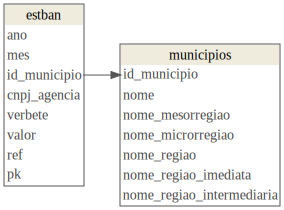
\includegraphics[width=8cm]{img/data_model.png}
  \end{center}
\end{figure}

\end{anexosenv}

% índice remissivo 
\phantompart
\printindex
